
\documentclass{standalone}

\usepackage{mathpazo}
\usepackage{tikz}
\usepackage{../../styles/tangocolors}

\begin{document}

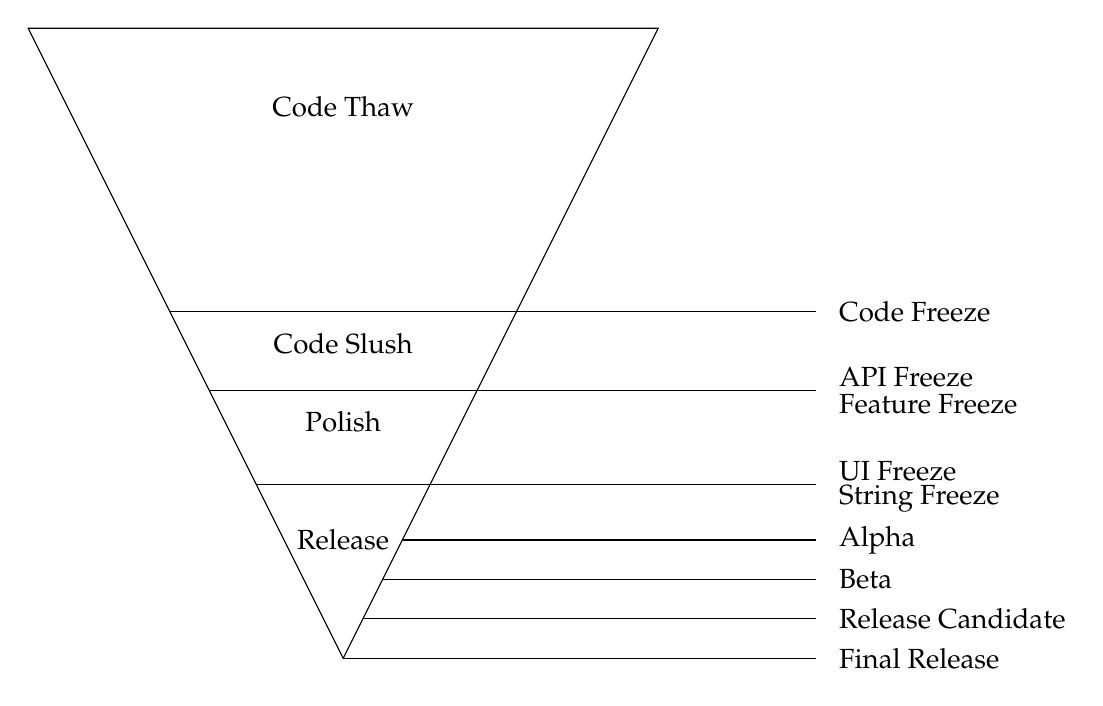
\begin{tikzpicture}
  \draw (0cm, 0cm) -- (8cm, 0cm) -- (4cm, -8cm) -- cycle;
  \draw (1.8cm, -3.6cm) -- (10cm, -3.6cm);
  \draw (2.3cm, -4.6cm) -- (10cm, -4.6cm);
  \draw (2.9cm, -5.8cm) -- (10cm, -5.8cm);

  \node[align=center] at (4cm, -1cm) {Code Thaw};
  \node[align=center] at (4cm, -4cm) {Code Slush};
  \node[align=center] at (4cm, -5cm) {Polish};
  \node[align=center] at (4cm, -6.5cm) {Release};

  \node[above=0pt, right=5pt] at (10cm, -3.6cm) {Code Freeze};
  \node[above=5pt, right=5pt] at (10cm, -4.6cm) {API Freeze};
  \node[below=5pt, right=5pt] at (10cm, -4.6cm) {Feature Freeze};
  \node[above=5pt, right=5pt] at (10cm, -5.8cm) {UI Freeze};
  \node[below=5pt, right=5pt] at (10cm, -5.8cm) {String Freeze};

  \node[right=5pt] at (10cm, -6.5cm) {Alpha};
  \node[right=5pt] at (10cm, -7.0cm) {Beta};
  \node[right=5pt] at (10cm, -7.5cm) {Release Candidate};
  \node[right=5pt] at (10cm, -8.0cm) {Final Release};

  \draw (4.75cm, -6.5cm) -- (10cm, -6.5cm);
  \draw (4.50cm, -7.0cm) -- (10cm, -7.0cm);
  \draw (4.25cm, -7.5cm) -- (10cm, -7.5cm);
  \draw (4cm, -8.0cm) -- (10cm, -8.0cm);

\end{tikzpicture}

\end{document}
